\documentclass[border=10pt]{standalone}

\usepackage{tikz}
\usepackage{tikzsymbols}
\usetikzlibrary{calc,patterns,shapes.geometric}

\def\centerarc[#1](#2)(#3:#4:#5){\draw[#1] ($(#2)+({#5*cos(#3)},{#5*sin(#3)})$) arc (#3:#4:#5);}

\begin{document}
	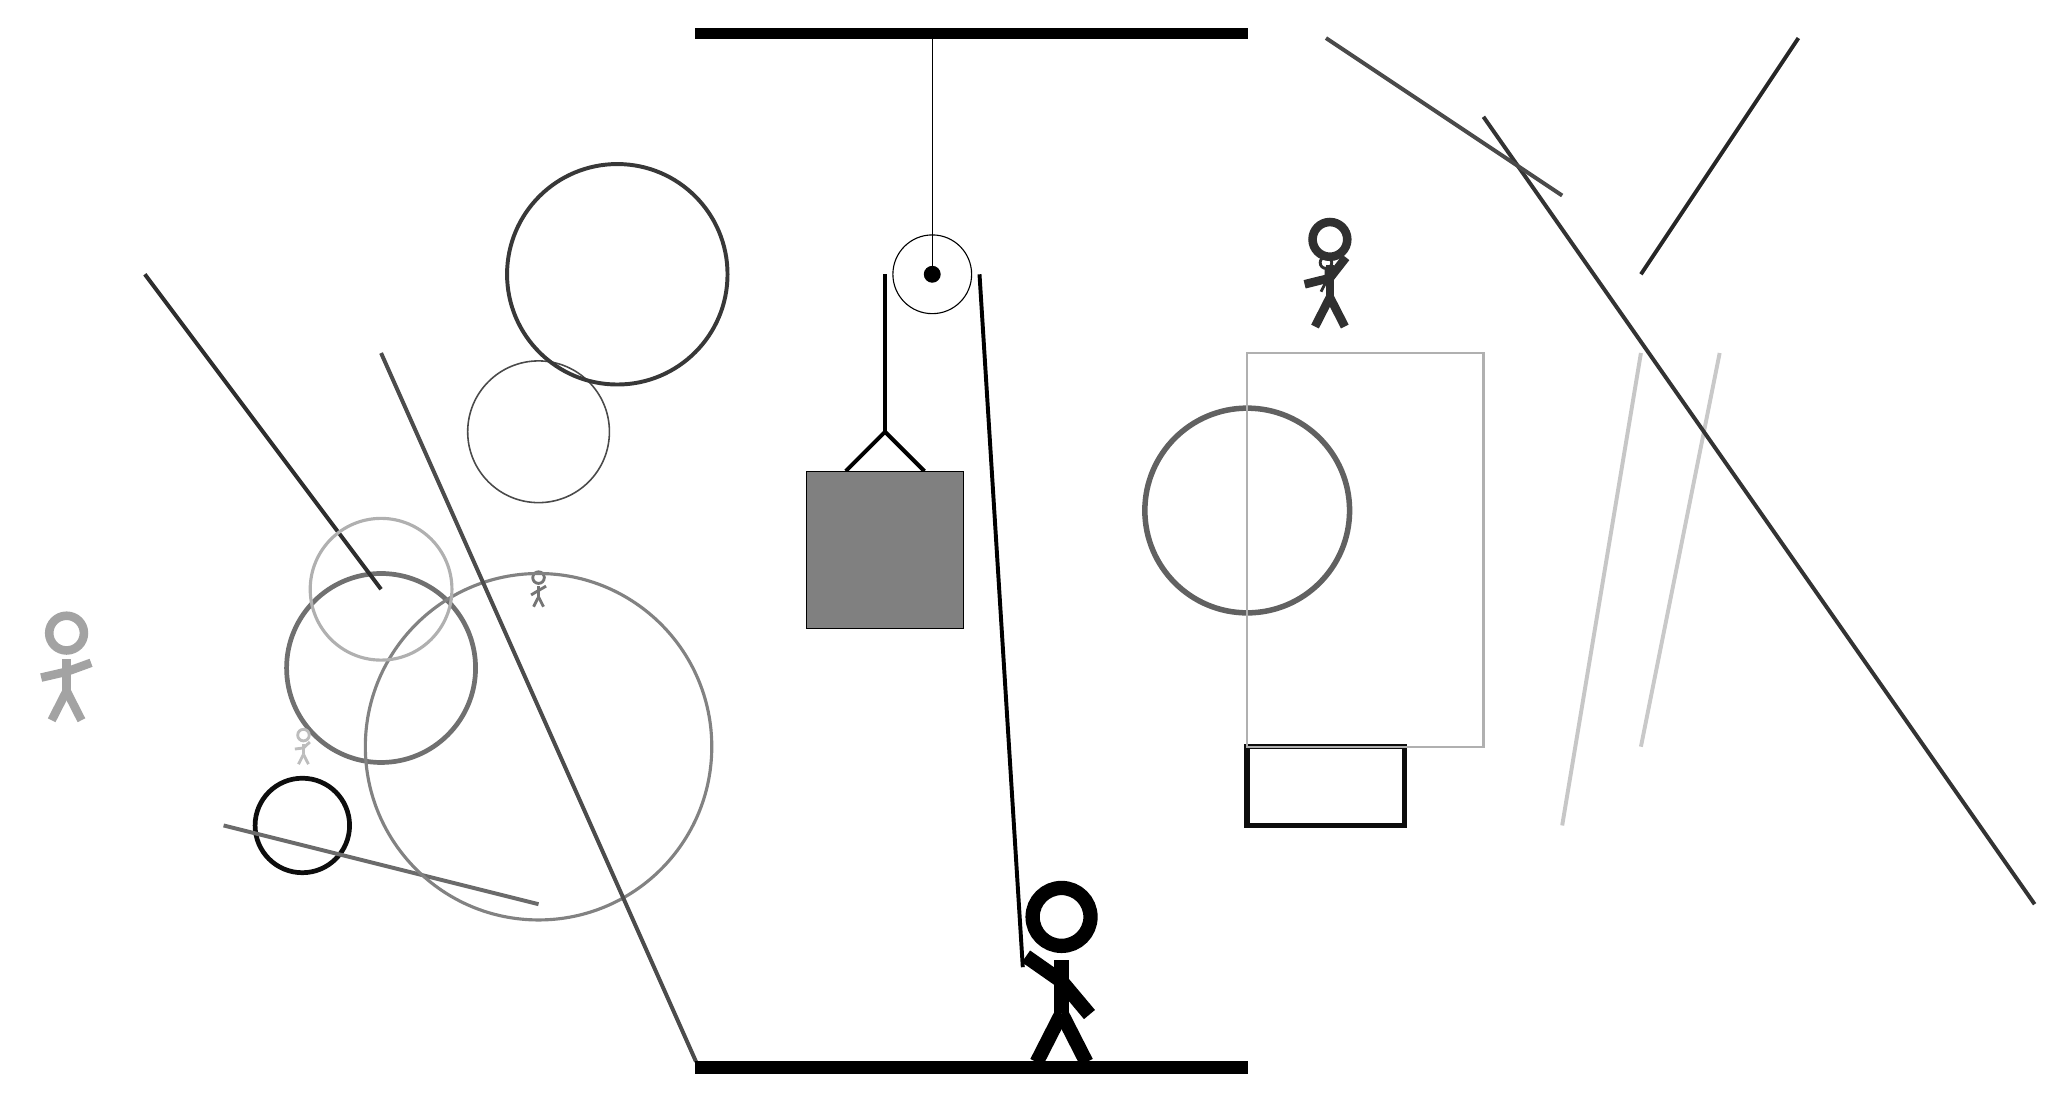
\begin{tikzpicture}
		%%%%% START %%%%%
		
		\draw[fill=black] (-2, 10) rectangle (5, 10.125);
		
		\draw (1, 7) circle (0.5);
		\draw[fill=black] (1, 7) circle (0.1);
		\draw (1, 10) -- (1, 7);
		
		\draw[line width=0.5mm, color=black!21](10, 1) -- (11, 6);
		
		\draw [line width=0.6mm, color=black!56](-6, 2) circle (1.2);
		\draw [line width=0.7mm, color=black!62](5, 4) circle (1.3);
		\draw[line width=0.5mm, color=black!82](-6, 3) -- (-9, 7);
		\draw[line width=0.7mm, color=black!95] (7, 0) rectangle (5, 1);
		\node[line width=0.5mm, color=black!26] at (-7, 1) {\Strichmaxerl[2][7][43]};
		
		\node[line width=0.2mm, color=black!54] at (-4, 3) {\Strichmaxerl[2][31][30]};
		\draw[line width=0.5mm, color=black!80](8, 9) -- (15, -1);
		\draw[line width=0.5mm, color=black!85](10, 7) -- (12, 10);
		\draw [line width=0.6mm, color=black!95](-7, 0) circle (0.6);
		\draw[line width=0.5mm, color=black!22](9, 0) -- (10, 6);
		\draw [line width=0.2mm, color=black!71](-4, 5) circle (0.9);
		\draw[line width=0.3mm, color=black!31] (5, 6) rectangle (8, 1);
		\draw[line width=0.5mm, color=black!58](-4, -1) -- (-8, 0);
		\node[line width=0.2mm, color=black!81] at (6, 7) {\Strichmaxerl[6][14][52]};
		\draw [line width=0.4mm, color=black!49](-4, 1) circle (2.2);
		
		\draw [line width=0.4mm, color=black!31](-6, 3) circle (0.9);
		\draw [line width=0.5mm, color=black!78](-3, 7) circle (1.4);
		\draw[line width=0.5mm, color=black!71](6, 10) -- (9, 8);
		
		\node[line width=0.6mm, color=black!81] at (6, 7) {\Strichmaxerl[2][52][89]};
		\node[line width=0.2mm, color=black!36] at (-10, 2) {\Strichmaxerl[6][13][20]};
		\draw[line width=0.5mm, color=black!70](-6, 6) -- (-2, -3);
		
		
		\draw[line width=0.5mm] (-0.1, 4.5) -- (0.4, 5.0) -- (0.9, 4.5);
		\draw[fill=black!50] (-0.6, 4.5) rectangle (1.4, 2.5);
		
		\draw[line width=0.5mm] (0.4, 7) -- (0.4, 5.0);
		\centerarc[line width=0.5mm](1, 7)(0:180:0.6);
		\draw[line width=0.5mm](1.6, 7) -- (2.15, -1.8);
		
		\node at (2.6, -1.9) {\Strichmaxerl[10][-35][-50]};
		
		\draw[fill=black] (-2, -3) rectangle (5, -3.15);
		
		%%%%% END %%%%%
	\end{tikzpicture}
\end{document}